\section{Stream-API}
\verb|java.util.stream.*|\\
Wird für deklarative Abfragen von Collections gebraucht. Code definiert, \textbf{was} gesucht wird, nicht \textbf{wie}.
Das Framework arbeitet sehr intensiv mit Lambdas und ist komplett unabhängig von Input/Output-Streams.\\
Basisschnittstellen:
\begin{itemize}
    \itemsep0em
    \item Für Referenzdatentypen
    \begin{itemize}
        \item \verb|Stream<T>|
    \end{itemize}
    \item Für primitive Datentypen
    \begin{itemize}
        \itemsep0em
        \item \verb|IntStream|
        \item \verb|LongStream|
        \item \verb|DoubleStream|
    \end{itemize}
\end{itemize}

\subsection{Endliche Quellen}
\begin{tabular}{l l}
    \verb|list.stream()              | & Liefert Stream anh. Collection \\
    \verb|Arrays.stream(array)       | & Liefert Stream anh. Array \\
    \verb|IntStream.range(1, 100)    | & Zahlen von 1 bis 100 \\
    \verb|Stream.of(2, 3, 5, 7)      | & eigene Aufzählung \\
    \verb|Stream.concat(strm1, strm2)| & Verketteter Stream \\
\end{tabular}

\subsection{Unendliche Quellen}
\verb|generate()| \\
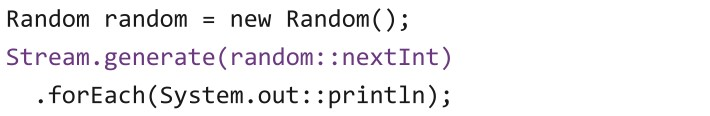
\includegraphics[width=0.7\linewidth]{pictures/generate.jpg}

\verb|iterate()| \\
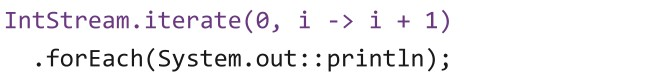
\includegraphics[width=0.6\linewidth]{pictures/iterate.jpg}

\subsection{Zwischenoperationen}
\begin{tabular}{l l}
    \verb|filter(Predicate) | & Filtern mit Lambda \\
    \verb|map(Function)     | & Mappen mit Lambda \\
    \verb|mapToInt(Function)| & Mappen mit \verb|int,long, double| \\
    \verb|sorted(Comparator)| & Sortieren mit Comparator \\
    \verb|distinct()        | & Duplikate entfernen gemäss \verb|equals()| \\
    \verb|limit(long n)     | & n-Elemente liefern \\
    \verb|skip(long n)      | & n-Elemente überspringen \\
\end{tabular}
Zwischenoperationen dürfen die Collection \textbf{nicht ändern} und sie dürfen keine Abhängigkeit zu äusseren, änderbaren Variablen haben.

\subsection{Terminaloperationen}
Der Stream ist nach einem solchen Aufruf fertig
\begin{tabular}{l l}
    \verb|forEach(Consumer)     | & Pro Element Operation anwenden \\
    \verb|count()               | & Anzahl Elemente \\
    \verb|min(),max()           | & bei \verb|Stream<T>| Comparator-Arg. erf. \\
    \verb|average(), sum()      | & Nur bei in/long/double-Stream \\
    \verb|findAny(), findFirst()| & Gibt irgendein/erstes Element zurück \\
    \verb|collect()|              & Rückumwandlung zu Collection \\
    \verb|toArray()|              & Rückumwandlung zu Array \\
\end{tabular}

\subsubsection{Collectors}
\verb|Collectors.toList()| $\rightarrow$ in Liste abbilden

\verb|Collectors.toCollection(TreeSet::new)| \\
$\hookrightarrow$ in beliebige Collection abbilden (Konstruktorreferenz)

\verb|Collectors.groupingBy(key, aggregator)|:
\begin{itemize}
    \itemsep0em
    \item Gruppierung mit opt. Aggregator
    \item Aggregator: averaging, summing, counting
    \item Liefert HashMap als Rückgabewert
\end{itemize}

\subsection{Funktionsschnittstellen}
\subsubsection{Vordefinierte}
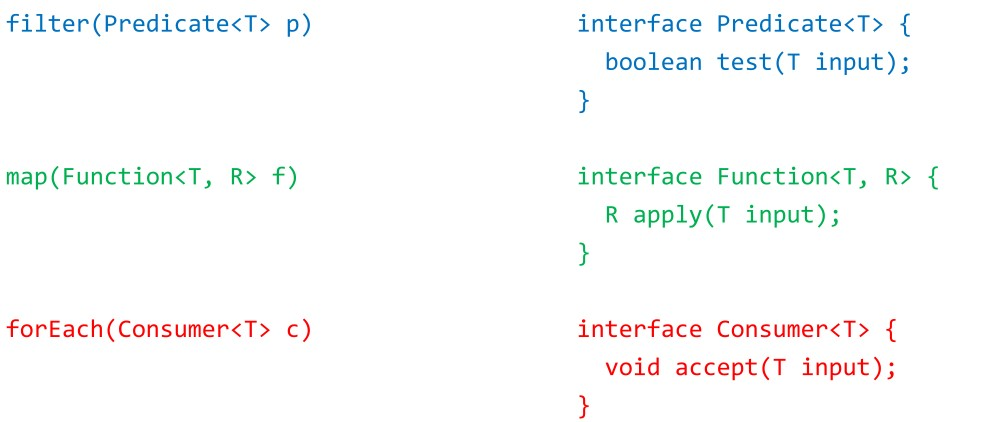
\includegraphics[width=\linewidth]{pictures/funktionsschnitt-vordef.jpg}

\subsubsection{Optional-Wrapper}
\verb|average(), min(), max(), findAny(), findFirst()| \\
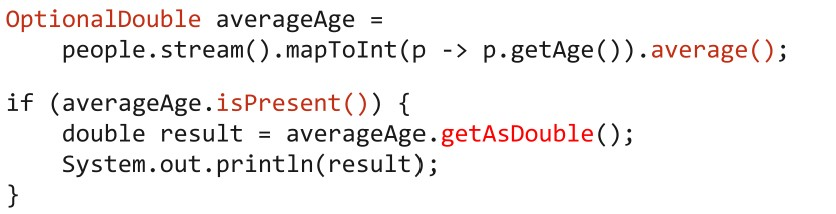
\includegraphics[width=\linewidth]{pictures/optional-wrapper.jpg}

\subsubsection{Matching}
\verb|allMatch(), anyMatch(), noneMatch()| \\
Prüfen, ob das Prädikat auf alle / irgendein/ kein Element zutrifft \\
\verb|boolean 18plus = ppl.stream().allMatch(p->p.getAge >= 18);|